\section{Durchführung}
\label{sec:Durchführung}

\subsection{Vorbereitungsaufgaben}
%\label{subsec:Vorbereitungsaufgaben} gibt in V353 keine Vorbereitungsaufgaben

In V107 sind zwei Vorbereitungsaufgaben vorgesehen.

\textbf{1. Wann wird eine Strömung als "laminar" bezeichnet?} \\
Eine laminare Strömung ist wirbelfrei und lässt sich an der Reynolds-Zahl erkennen, siehe Abschnitt 
Theorie \ref{subsec:Reynolds-Zahl}.



\textbf{2. Die Dichte und dynamische Viskosität von destilliertem Wasser als Funktion der Temperatur}\\
\begin{figure}
    
    \centering
    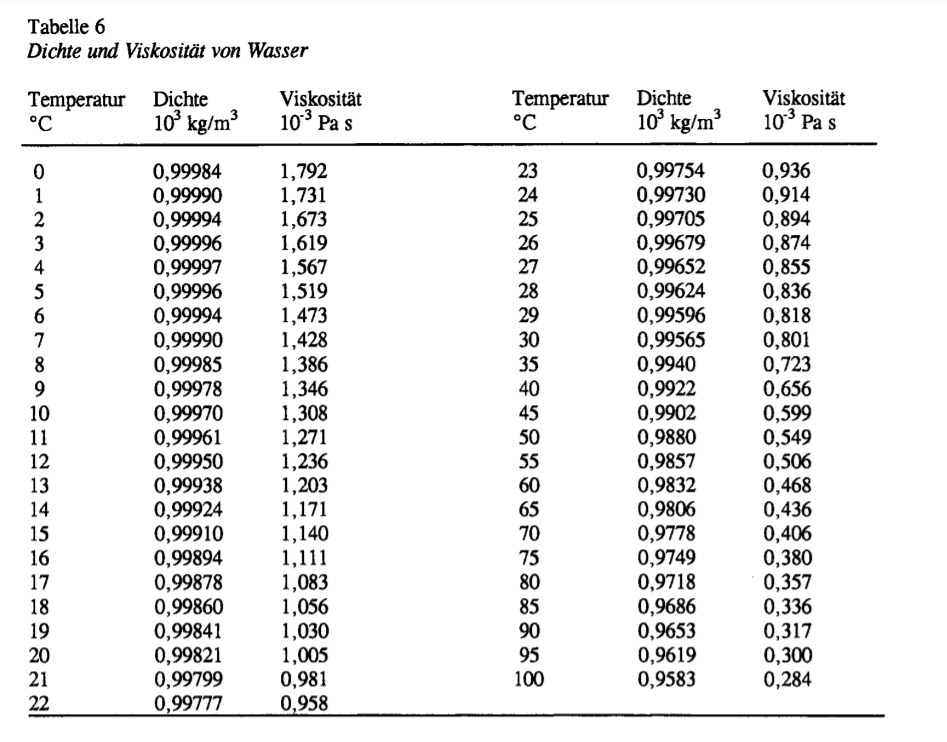
\includegraphics[height=3cm]{content/DichteWasser.png}
    \caption{Quelle: angegebene Literatur}
    \label{fig:DichteWasser}
\end{figure}




\subsection{Aufgaben}
\label{subsec:Aufgaben}

Es soll mit Hilfe der Reynoldschen Zahl bestimmt werden, ob die Strömung laminar ist.

Darüber hinaus wird mit Hilfe der genommenen Messdaten die Temperaturabhängigkeit der Viskosität von
destilliertem Wasser berechnet. 

Im ersten Teil des Versuchs lässt man zwei Kugeln verschiedener Größe wiederholt das Viskosimeter 
passieren und misst die Zeit, die sie für das Durchqueren einer markierten Strecke bestimmter Länge brauchen. \\
Das Wasser ist hier bei Raumtemperatur und es werden je Kugel 10 Messungen durchgeführt, die jeweils Hin- und Rückweg 
beinhalten.

Im zweiten Teil wird das Wasser nun langsam bis auf 50 Grad Celsius aufgeheizt, während zwischendurch 
insgesamt bei verschiedenen Temperaturen mindestens 10 Messungen mit der größeren Kugel durchgeführt werden. 




\subsection{Aufbau}
\label{subsec:Aufbau}

Das Höppler-Viskosimeter ist in \ref{fig:aufbau} zu sehen.

\begin{figure}
    
    \centering
    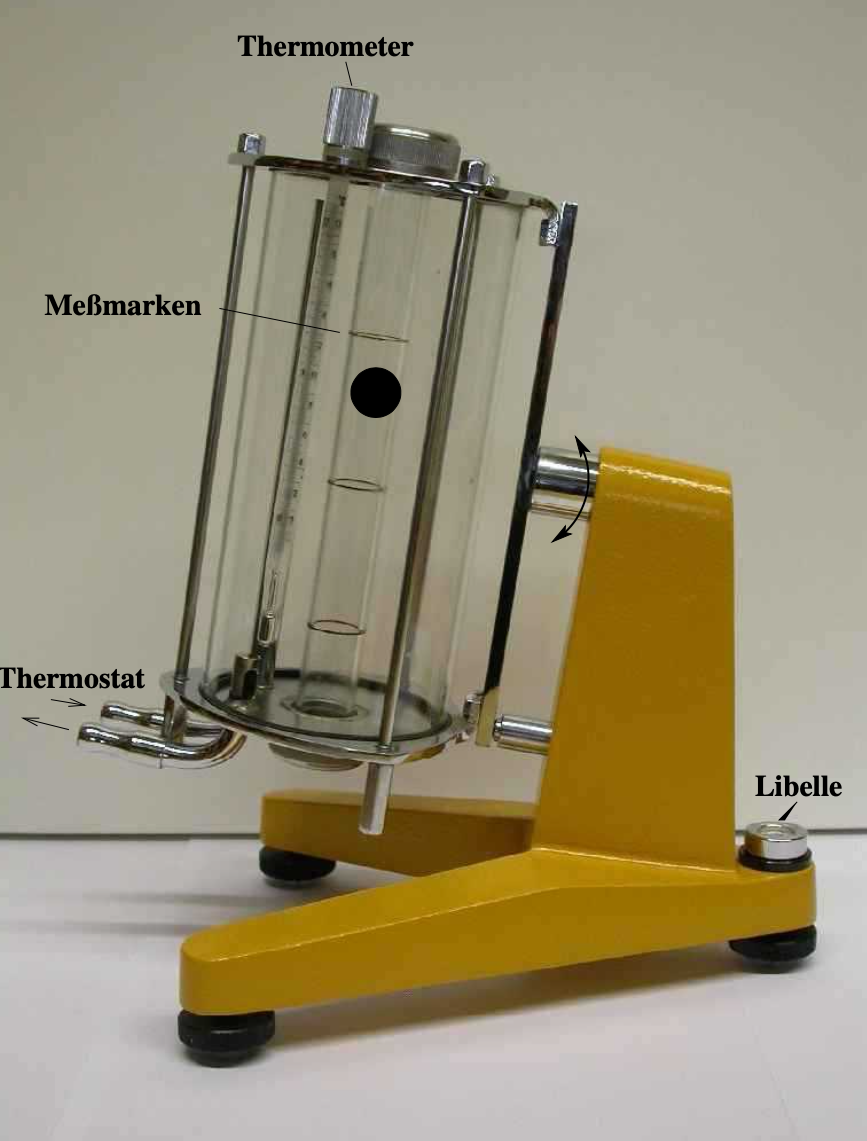
\includegraphics[height=3cm]{content/hoeppler.png}
    \caption{Das Hoeppler-Viskosimeter)}
    \label{fig:aufbau}
\end{figure}